\section{Design}

The proposed system follows the structure represented in the Fig. \ref{fig:infra_scheme} and it is composed of two modules. The \emph{perception} module is responsible for performing the \emph{vision tasks}. Therefore, it determines, with the maximum possible accuracy, the position of every person found inside the color image. It also discerns which of these persons is the one to be followed, in case she is seen. The \emph{actuation} module reads that output from the percpetion module and sends suitable movement commands to the robot.

\begin{figure}[h]
	\centering
	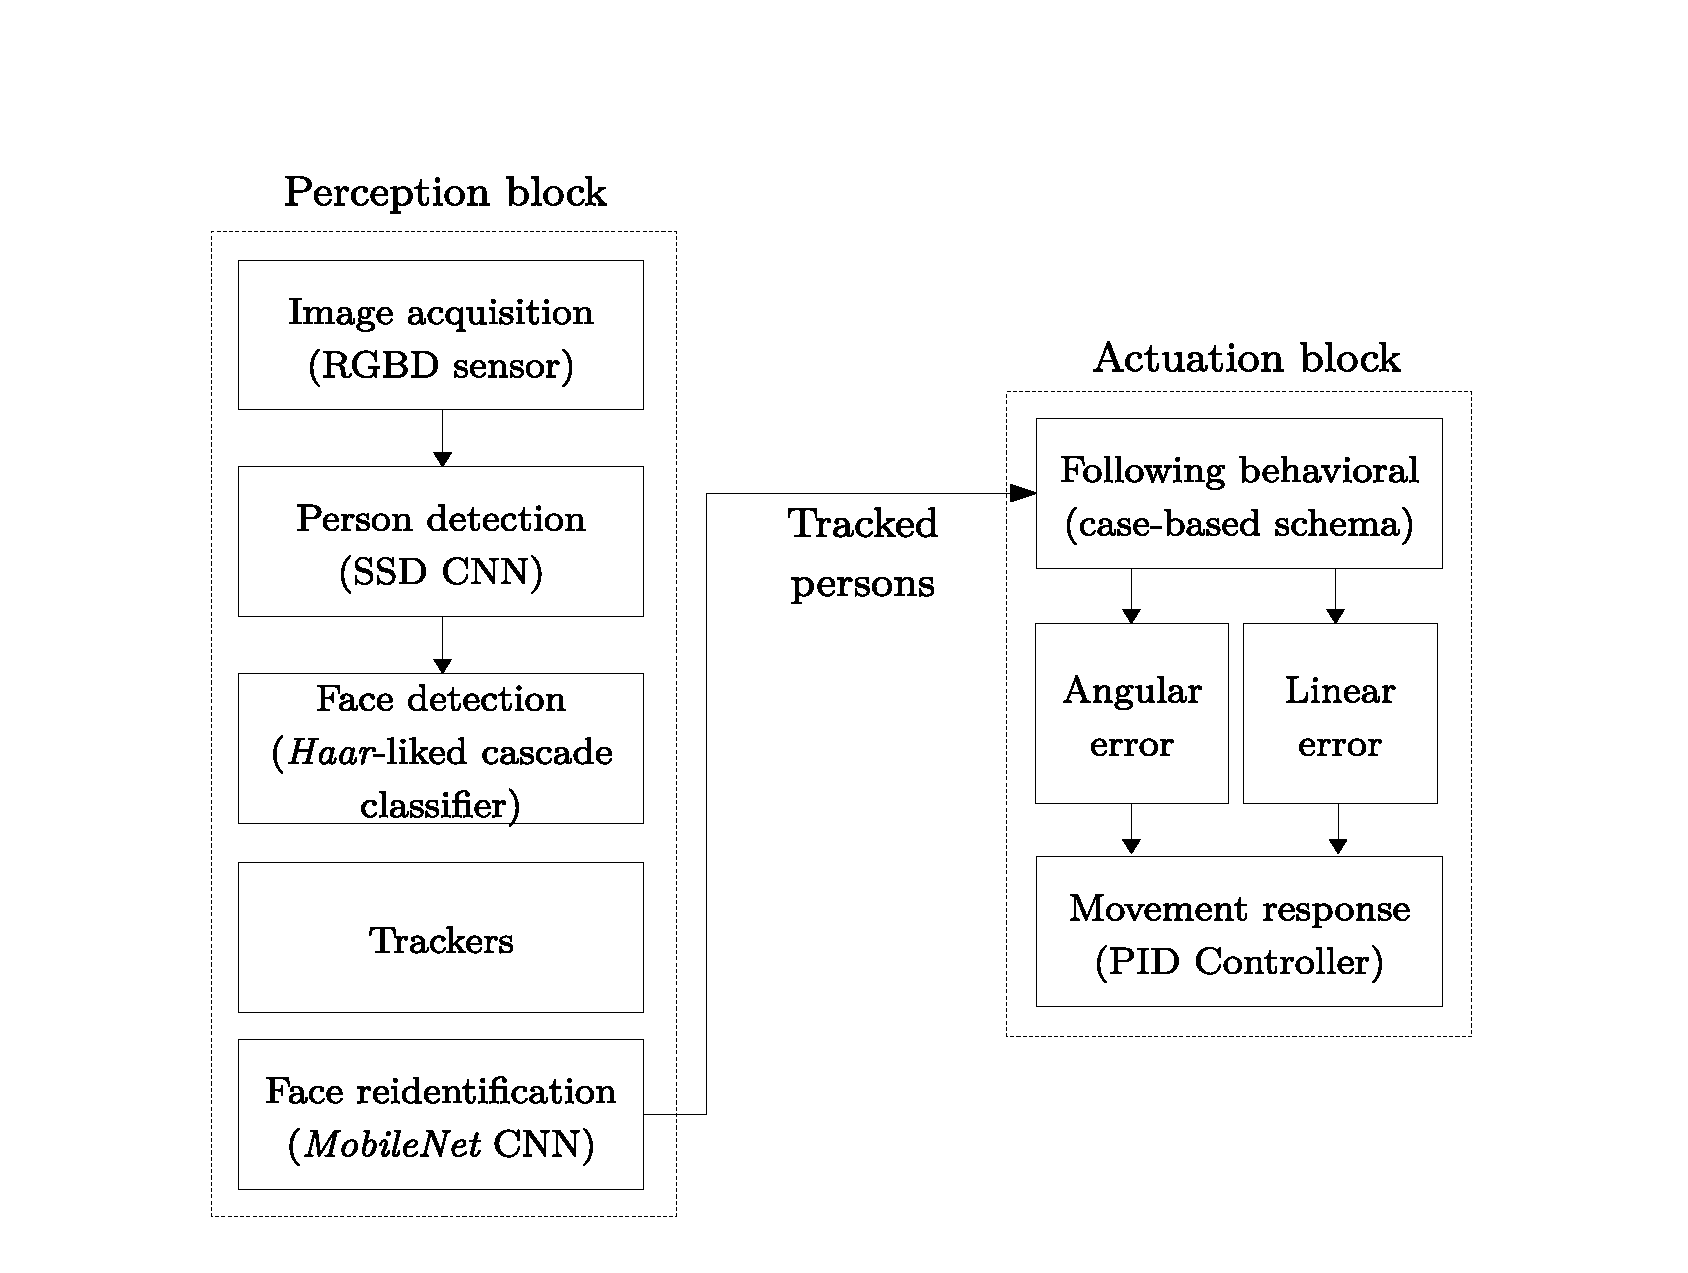
\includegraphics[width=12cm]{images/system_schema}
	\caption{General design of the proposed system.}
	\label{fig:infra_scheme}
\end{figure}

These mentioned modules run on a computer, connected to both the RGBD sensor driver and the robot driver. They have been implemented in Python language as concurrent threads inside a single program. Both threads run iterative iterations at a certain controlled frequency. In case of slow computer the frequency may be lower than the regular one, and so, the system is designed to run properly on different hardware specifications of the base PC.